\begin{appendices}
	
\section*{mAP (mean Average Precision)}\label{app:mAP}
La mAP est une mesure de précision pour les algorithmes de détection d'objet. La mAP correspond de manière générale à la moyenne de l'AP obtenu sur différents objets et à différents paramètres. Son calcul dépend du contexte et de la technique de comparaison.\\
L'Average Precision (AP) se calcule en se basant sur la précision, le rappel et l'Intersection over Union. 
\begin{figure}[!htbp]
\center
	\subfloat{{\includegraphics[scale=0.25]{truefalsepositivesnegatives.png}}}
\caption{Schéma vrais/faux positifs/négatifs}
\label{fig:schema_vraifaux}
\end{figure}
\FloatBarrier
La précision correspond à la proportion de vrais positifs (VP) parmi l'ensemble des vrais positifs et des faux positifs (FP). 
$$precision = \frac{VP}{VP+FP}$$
Le rappel correspond à la proportion de vrais positifs parmi l'ensemble des vrais positifs et des faux négatifs (FN).
$$rappel = \frac{VP}{VP+FN}$$
On trace ensuite la courbe représentant la précision en fonction du rappel : 
\begin{figure}[!htbp]
\center
	\subfloat{{\includegraphics[scale=0.2]{prcurve.png}}}
\caption{Tracé de la coubre Precision-Recall ou PR curve}
\label{fig:trace_prcurve}
\end{figure}
\FloatBarrier
L'AP correspond à l'aire sous cette courbe Precision-Rappel (PR curve). 
$$\int_{0}^{1} f_{PR}(rappel) \hspace{0.1cm} d(rappel)$$

	

	
\clearpage
\section*{Diagramme UML global}\label{app:UMLGlobal}
\begin{figure}[!htbp]
	\center
		\subfloat{{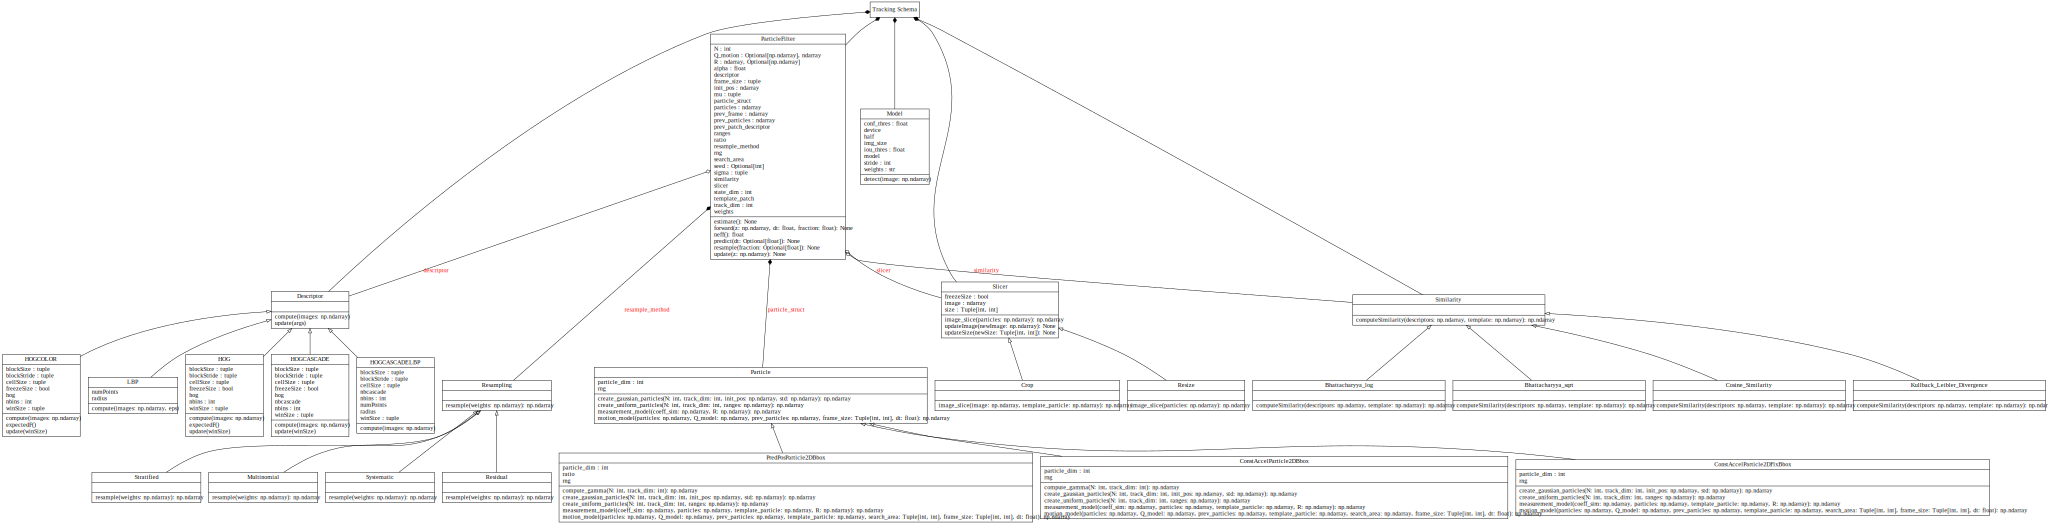
\includegraphics[scale=0.1,angle=90,origin=c]{classes.png}}}
	\caption{Diagramme UML des classes globales (\href{https://raw.githubusercontent.com/gabriel-combe/Cuttlefish_Tracker/main/rapport/UML/classes.svg}{lien vers l'image SVG}, zoomer sur l'image SVG pour avoir plus de détails).}
	\label{fig:uml_diagram_classes}
\end{figure}
\FloatBarrier
	

\clearpage
\section*{Diagramme UML mesure de similarité}\label{app:UMLSimilarity}
\begin{figure}[!htbp]
	\center
		\subfloat{{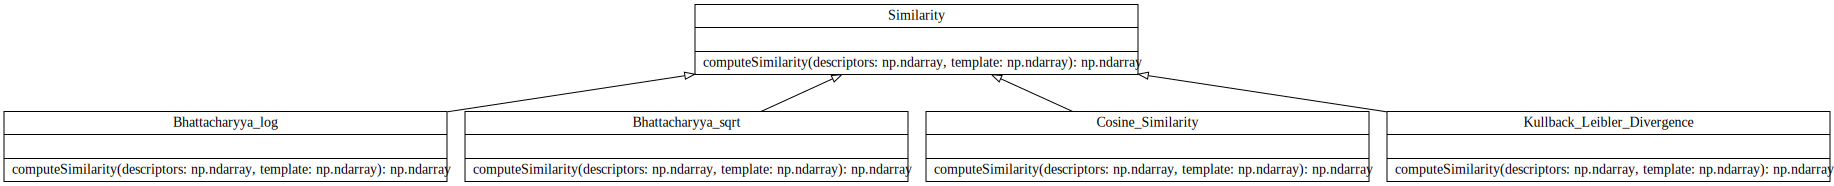
\includegraphics[scale=0.26,angle=90,origin=c]{similarity.png}}}
	\caption{Diagramme UML de la classe Similarity (\href{https://raw.githubusercontent.com/gabriel-combe/Cuttlefish_Tracker/main/rapport/UML/similarity.svg}{lien vers l'image SVG}, zoomer sur l'image SVG pour avoir plus de détails).}
	\label{fig:uml_diagram_similarity}
\end{figure}
\FloatBarrier


\clearpage
\section*{Diagramme UML filtre à particule}\label{app:UMLParticleFilter}
\begin{figure}[!htbp]
	\center
		\subfloat{{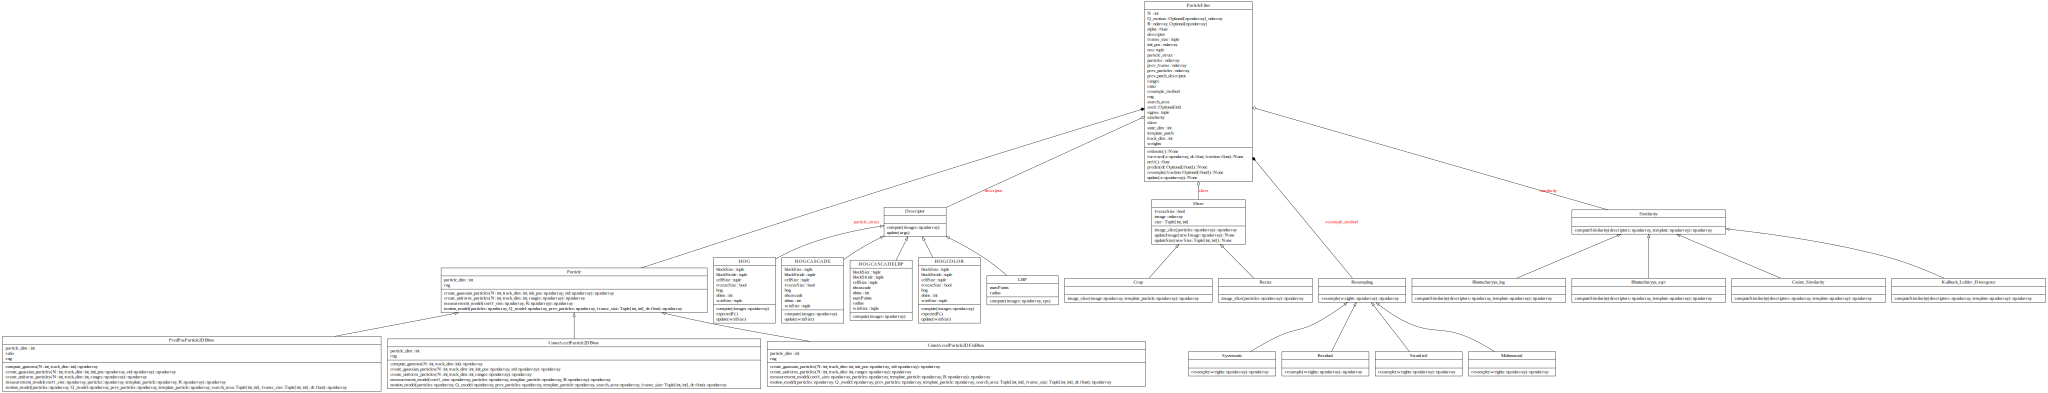
\includegraphics[scale=0.081,angle=90,origin=c]{particlefilter.png}}}
	\caption{Diagramme UML de la classe ParticleFilter (\href{https://raw.githubusercontent.com/gabriel-combe/Cuttlefish_Tracker/main/rapport/UML/particlefilter.svg}{lien vers l'image SVG}, zoomer sur l'image SVG pour avoir plus de détails).}
	\label{fig:uml_diagram_particlefilter}
\end{figure}
\FloatBarrier
	
	
\clearpage
\section*{VAE (Variational Autoencoder)}\label{app:variational_autoencoder}
Les VAE, ou Variational Autoencoder, sont des réseaux de neurones qui essayent d'estimer une distribution probabiliste avec seulement un nombre limité d'échantillons provenant de cette distribution.\\
Ce genre de réseaux de neurones est divisé en deux parties:\\
\begin{itemize}
	\item \emph{Encodeur}\\
	Pour une donnée $x$, l'encodeur va projeter/compresser $x$ dans un espace de représentation plus petit (espace latent).\\
	L'encodeur a pour objectif de représenter $x$ de façon optimisée, et de conserver les informations les plus importantes.\\
	\item \emph{Décodeur}\\
	Pour une représentation issue de l'espace latent, le décodeur va essayer de décompresser/reconstruire $x$ en minimisant les pertes d'information.\\
	Le décodeur a pour objectif de produire une donnée $x'$ la plus similaire possible à $x$.\\
\end{itemize}
	
Le schéma global est illustré en figure \ref{fig:vae_scheme}.
\begin{figure}[!htbp]
\center
	\subfloat{{\includegraphics[scale=0.3]{VAE_Basic.png}}}
\caption{Schéma basique d'un VAE.}
\label{fig:vae_scheme}
\end{figure}
\FloatBarrier

\end{appendices}

\clearpage
